% \iffalse meta-comment
%
% Copyright (C) 2020 by David Gustavsson
%
% This file may be distributed and/or modified under the
% conditions of the LaTeX Project Public License, either
% version 1.3 of this license or (at your option) any later
% version. The latest version of this license is in:
%
% http://www.latex-project.org/lppl.txt
%
% and version 1.3 or later is part of all distributions of
% LaTeX version 2005/12/01 or later.
%
% \fi
%
% \iffalse
%<package>\NeedsTeXFormat{LaTeX2e}[2020/02/02]
%<package>\ProvidesPackage{datax}
%<package>      [2020/11/29 v1.1.1 data import into LaTeX]
%<package>\RequirePackage{pgfkeys}
%<package>\RequirePackage{pgfopts}
%
%<*driver>
\begin{filecontents}[overwrite]{datax-example-data.tex}
        \pgfkeyssetvalue{/datax/s}{A literal string}
        \pgfkeyssetvalue{/datax/x}{\num{2.4}}
        \pgfkeyssetvalue{/datax/c}{\SI{3e8}{\meter\per\second}}
\end{filecontents}
\begin{filecontents*}[overwrite]{datax-example-script.jl}
        #!julia
        using LaTeXDatax, Unitful

        s = "A literal string";
        x = 2.4;
        c = 3e8u"m/s";

        @datax s x c
\end{filecontents*}
\documentclass{ltxdoc}
\usepackage[dataxfile=datax-example-data.tex]{datax}
\usepackage{booktabs}
\usepackage{siunitx}
\usepackage[hidelinks]{hyperref}
\usepackage{tikz}
\usepackage{float}
\usepackage{listings}
\usepackage{microtype}

\newfloat{lstfloat}{htbp}{lop}
\floatname{lstfloat}{Listing}
\def\lstfloatautorefname{Listing}

\EnableCrossrefs
\CodelineIndex
\RecordChanges
\begin{document}
\DocInput{datax.dtx}
\end{document}
%</driver>
% \fi
%
%\CheckSum{29}
%
% \CharacterTable
%  {Upper-case    \A\B\C\D\E\F\G\H\I\J\K\L\M\N\O\P\Q\R\S\T\U\V\W\X\Y\Z
%   Lower-case    \a\b\c\d\e\f\g\h\i\j\k\l\m\n\o\p\q\r\s\t\u\v\w\x\y\z
%   Digits        \0\1\2\3\4\5\6\7\8\9
%   Exclamation   \!     Double quote  \"     Hash (number) \#
%   Dollar        \$     Percent       \%     Ampersand     \&
%   Acute accent  \'     Left paren    \(     Right paren   \)
%   Asterisk      \*     Plus          \+     Comma         \,
%   Minus         \-     Point         \.     Solidus       \/
%   Colon         \:     Semicolon     \;     Less than     \<
%   Equals        \=     Greater than  \>     Question mark \?
%   Commercial at \@     Left bracket  \[     Backslash     \\
%   Right bracket \]     Circumflex    \^     Underscore    \_
%   Grave accent  \`     Left brace    \{     Vertical bar  \|
%   Right brace   \}     Tilde         \~}
%
% \changes{v1.0}{2020/11/15}{Initial version}
% \changes{v1.1}{2020/11/17}{Polishing for release}
% \changes{v1.1.1}{2020/11/29}{Renaming the plugins, adding Python support}
%
% \GetFileInfo{datax.sty}
% \DoNotIndex{}
%
% \title{The \textsf{datax} package\thanks{This document corresponds to
% \textsf{datax}~\fileversion, dated~\filedate.}} \author{David Gustavsson
% \href{mailto:david.e.gustavsson@gmail.com}{\texttt{david.e.gustavsson@gmail.com}}}
%
% \maketitle {\centering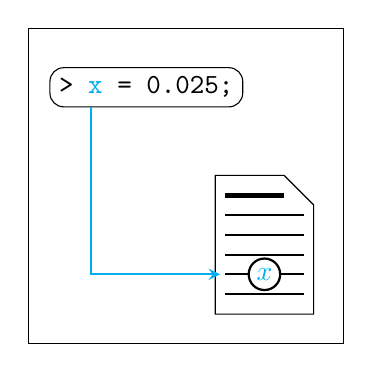
\begin{tikzpicture}
	\definecolor{variablecolor}{named}{cyan}
	\draw (-2,-2) rectangle (2,2);

	%  Script {{{
	\begin{scope}[shift={(-0.5,1.25)}]
		\node[draw=black,rounded corners=5] (code) at (0,0) {\texttt{> {\color{variablecolor}x} = 0.025;}};
	\end{scope}
	%  }}}

	%  Document {{{
	\begin{scope}[shift={(1,-0.75)}, scale=1.25]
		\draw (0.2,0.705) -| (-0.5,-0.705) -| (0.5,0.405) -- cycle;
		\draw[line width=2] (-0.4,0.5) -- (0.2,0.5);
		\draw[thick] %
		(-0.4,0.3) -- (0.4,0.3) %
		(-0.4,0.1) -- (0.4,0.1) %
		(-0.4,-0.1) -- (0.4,-0.1) %
		(-0.4,-0.3) -- node[inner sep=1.5,circle,midway,variablecolor,draw=black,fill=white](variable) {\(x\)} (0.4,-0.3) %
		(-0.4,-0.5) -- (0.4,-0.5) %
		;
	\end{scope}
	%  }}}

	\draw[thick,-stealth, shorten >=10, variablecolor] (code.-160) |- (variable);

\end{tikzpicture}
\\}
%
% \section{Motivation}
% \textsf{datax} allows you to export data from your scripts, and import them
% as literal strings or \textsf{siunitx} commands. If the scripts or the data
% on which they operate change, the printed data will update as well. This is
% analogous to how the author uses \textsf{graphicx} to programmatically
% generate graphics and include in a document.
%
% An alternative is to simply print |\def|s, which scales poorly (but is
% similar to how this package works under the hood).  Or using something like
% \textsf{csvread}, which seems overkill for individual data points, and can be
% quite difficult to index into.
%
% \textsf{datax} is intended to work as an extension of your variable name
% space from scripts to your document: you should simply be able to call your
% variables by the same name in \LaTeX{} as in your scripts.
%
% \section{Installation}
% If you have a \LaTeX{} package manager, like texlive or miktex, use it to
% download the package from ctan.  Otherwise, download the repository and place
% |datax.sty| in a place where \LaTeX{} can find it (often
% |~/texmf/tex/latex/datax/datax.sty|). Run |texhash| if needed.
%
% \section{Usage}
% The package is loaded with |\usepackage[dataxfile=|\meta{data.tex}|]{datax}|,
% which reads the file specified as \meta{dataxfile}.  From then on data can be
% inserted as |\datax|\marg{tag}\DescribeMacro{\datax}. If, for instance, the
% file |data.tex| contains references to a string \(s\), a number \(x\) and a
% physical constant \(c\), then the macro produces the output in
% table~\ref{tab:outputs}.
%
% I highly recommend using \textsf{siunitx} (in general, but with
% \textsf{datax} in particular).  It is of course possible to use the literal
% string function to circumvent siunitx and make \textsf{datax} print numbers
% without |\num| and |\SI|, which is why \textsf{siunitx} is not loaded as a
% prerequisite, but I have deliberately chosen to use these commands per
% default when printing numbers and quantities because it looks much better.
%
% \begin{table}
%     \centering
%     \caption{Outputs from the \texttt{\textbackslash{}datax}
%     command}\label{tab:outputs}
%     \begin{tabular}{rl}\toprule
%         Input & Output \\\midrule
%         |\datax{s}| & \datax{s} \\
%         |\datax{x}| & \datax{x} \\
%         |\datax{c}| & \datax{c} \\
%         |\datax{undefined}| & \datax{undefined} \\
%         \bottomrule
%     \end{tabular}
% \end{table}
%
% \section{Interactions}
% Technically, \textsf{datax} only needs a data file consisting of a number of
% assignments: |\pgfkeyssetvalue{/datax/|\meta{tag}|}{|\meta{value}|}| but of
% course the entire point of the package is automation. For this, you need an
% interaction plugin for your script language. If your language is not listed
% in table~\ref{tab:plugins}, you might need to write this plugin for yourself,
% or request it.
%
% Installation instructions and usage documentation is available at the
% respective repositories. In general these plugins are installed using the
% language's default plugin manager.
%
% \begin{table}
% \centering
% \caption{Implemented language plugins}\label{tab:plugins}
% \begin{tabular}{rlp{5cm}}\toprule
% Language & Plugin & Comments\\\midrule
% |julia| & \href{https://github.com/Datax-package/LaTeXDatax.jl}{LaTeXDatax.jl} & By the present author \\
% |Matlab| & \href{https://github.com/Datax-package/LaTeXDatax.m}{LaTeXDatax.m} & By the present author \\
% |Python| & \href{https://github.com/Datax-package/LaTeXDatax.py}{LaTeXDatax.py} & By the present author \\
% \bottomrule
% \end{tabular}
% \end{table}
%
% Taking julia as an example, the variables in table~\ref{tab:outputs} could
% have been generated with the script in listing~\ref{list:julia}.

% \begin{lstfloat}
% \lstinputlisting[label=list:julia,caption={Example julia script to generate the outputs in table~\ref{tab:outputs}},
%                         language=python,frame=single,xleftmargin=.2\textwidth,xrightmargin=.2\textwidth]{datax-example-script.jl}
% \end{lstfloat}
%
%
% \StopEventually{\PrintIndex}
% \section{Implementation}
% Default data file name: \texttt{data.tex}
%    \begin{macrocode}
\pgfkeys{ /packageoptions/dataxfile/.initial=data.tex, }
\pgfkeys{ /packageoptions/siunitxoptions/.initial={}, }
%    \end{macrocode}
% Read any given options into family \texttt{/packageoptions/}. Then introduce
% family \texttt{/datax/} where all the variables will be stored.
%    \begin{macrocode}
\ProcessPgfPackageOptions{/packageoptions}

\pgfkeys{ /datax/.is family, datax, %
        .unknown/.code={ \pgfkeyssetvalue{ %
                        \pgfkeyscurrentpath/\pgfkeyscurrentname %
        }{ #1 } },
}

%    \end{macrocode}
% If data file exists, source it (storing all the variables in
% \texttt{/datax/}). Otherwise, throw a warning.
%    \begin{macrocode}
\def\dataxfile{./\pgfkeysvalueof{/packageoptions/dataxfile}}
\InputIfFileExists{%
        \dataxfile
        }{}{
        \PackageWarning{datax}{Cannot read file `\dataxfile'}
}
\newif\ifhassiunitx
\@ifpackageloaded{siunitx}{\hassiunitxtrue}{\hassiunitxfalse} 
%    \end{macrocode}
% \begin{macro}{\datax}
% Include datum. If the supplied tag is unused, print bold question marks (like
% |\ref|), and throw a warning.
%    \begin{macrocode}
\newcommand{\datax}[2][]{
        \pgfkeysifdefined{/datax/#2}{ %
                { %
                        \ifhassiunitx %
                                \sisetup{\pgfkeysvalueof{/packageoptions/siunitxoptions},#1}
                        \fi
                        \pgfkeysvalueof{/datax/#2} %
                } %
                }{ %
                \PackageWarning{datax}{Data value `#2' undefined}\textbf{??} %
        } %
}
%    \end{macrocode}
% \end{macro}
% \Finale
\endinput
